\chapter{Introduction}
Face is a particularly compelling biometric because it is used
everyday by everyone as the primary means for recognizing other
humans. Face recognition is an important capability of the human
perception system. Automated face recognition has become one of the
most important applications of image analysis and computer vision in
recent years. This has attracted the attention of many groups in
research institutes, academia, industries and governmental agencies.
This is obvious from the increased number of face recognition
contests such as FERET \cite{FERET2000}, XM2VTS \cite{Messer99},
FRVT 2000 \cite{FRVT2000}, FRVT 2002 \cite{FRVT2002}, FRVT 2006
\cite{FRVT2006}, and FRGC \cite{FRGC2005}.

There two major reasons for this enormous interest on face
recognition technology. The first reason is the existence of a large
number of forensic, security, and commercial applications. These
applications include video camera surveillance, access control, mug
shot identification (e.g., for issuing passport), design of human
computer interactions (HCI), multimedia communication, and
content-based image retrieval. The second reason is the availability
of technologies developed by researchers in the field of computer
vision, pattern recognition, image processing, and computer graphics
that has motivated the use of the technology for this purpose.

\section{Biometric System}
Recognizing the identity and authenticity of the people is the
fundamental process for many activities and applications in our
life. Biometric identification or biometrics refers to identifying
an individual based on his/her distinguishing characteristics. In
other words, biometrics is the science of identifying, or verifying
the identity of a person based on the behavioral or physiological
characteristics.

\subsection{History of Biometrics}
Possibly the first known example of the use of biometrics in
practice was the use of a form of finger printing in China in the
$14^{th}$ century, as reported by explorer Joao de Barros. He wrote
that the Chinese merchants were stamping children's palm prints and
footprints on paper with ink to distinguish the young children from
one another. This is one of the earliest known cases of biometrics
in use and is still being used today \cite{Garfinkel2000}.

Elsewhere in the world up until the late 1800s, identification
largely relied upon ``photographic memory.'' In the 1890s, an
anthropologist and police desk clerk in Paris named Alphonse
Bertillon sought to fix the problem of identifying convicted
criminals and turned biometrics into a distinct field of study. He
developed a method of multiple body measurements which got named
after him (Bertillonage). His system was used by police authorities
throughout the world, until it quickly faded when it was discovered
that some people shared the same measurements and based on the
measurements alone, two people could get treated as one. After the
failure of Bertillonage, the police started using finger printing,
which was developed by Richard Edward Henry of Scotland Yard,
essentially reverting to the same methods used by the Chinese for
years \cite{Garfinkel2000}.

\subsection{Types of Biometrics} In recent years biometrics moved from simple fingerprinting to many different methods that use
various physical and behavioral measures. The characteristics used
in each category are as follows:

\bi \item Physiological
    \bi
        \item Iris
        \item Fingerprint (including nail)
        \item Hand (including knuckle, palm, vascular)
        \item Face
        \item Retina
        \item DNA
        \item Vein
        \item Ear
        \item Even Odor, Sweat pore, Lips
    \ei
\item Behavioral
    \bi
        \item Signature
        \item Keystroke
        \item Voice
        \item Gait
    \ei
\ei

Among the biometric features/identifiers, Fingerprint, Face, Hand
geometry, Iris, Signature, and Voice are the most commonly used in
today's automated authentication systems. These biometrics received
more attentions than the others by researches in the filed of
computer science.

\subsection{Motivation and Overview} Biometric technologies are
becoming the foundation of an extensive array of highly secure
identification and personal verification solutions. As the level of
security breaches and transaction fraud increases, the need for
highly secure identification and personal verification technologies
is becoming apparent. The uses of biometrics have also increased
from just identification to verification as used in security systems
and more. Biometric-based solutions are able to provide for
confidential financial transactions and personal data privacy. The
need for biometrics can be found in federal, state and local
governments, in the military, and in commercial applications.
Enterprise-wide network security infrastructures, government IDs,
secure electronic banking, investing and other financial
transactions, retail sales, law enforcement, and health and social
services are already benefiting from these technologies.

\subsection{Biometric Authentication System} A biometric
authentication system can be considered as a pattern recognition
system with three modules consisting of: biometric sensor(s) to
collect the data from the biometric identifier, feature extractor,
and matcher. For example, in case of face recognition, the sensor is
a camera and the biometric identifier is a facial image. The task of
biometric authentication mainly is divided into two categories:

\bi
\item\textbf{Identification} is a closed-universe (one-to-many) comparing process
for a biometric sample from a given probe against all the known
biometric reference templates in the database. In other words, this
is the answer to the question ``Who am I?'' If the acquired sample
matches a stored template within an acceptable margin of error, then
the identity of the probe is matched to that of the previously
stored reference. During the matching process, a set of similarity
matching scores are obtained for the probe sample (i.e., one-to-many
comparison process). These similarity scores are numerically ranked
such that the highest similarity score is first and the smallest
similarity score is ranked $n$, where $n$ is the number of the
subjects enrolled in the database. In an ideal case, the highest
similarity score is the comparison of the claimed person's biometric
with the same person's biometric that was previously stored in the
database. The percentage of time that the highest similarity score
is the correct match for all individuals, is referred to as the
identification rate.

In order to evaluate the performance of identification, the
percentage of time when one of the top-$r$ matches is correct is
considered and called as ``Cumulative Match score''. In other words,
the ``Cumulative Match Score'' curve is the percentage of correct
identification versus the rank $r$. Usually the percentage of the
correct identification for the rank-one is reported as the
performance of a biometric system.

\item \textbf{Verification} is an open-universe (one-to-one) process of comparing a
submitted biometric sample against single biometric reference of a
single enrollee whose identity or role is being claimed. In other
words, this is the answer to the question, ``Am I who I claim I
am?'' The result of the verification is to confirm that the identity
is matched or not matched. During the process of matching, a
similarity score is computed by the biometric matcher; if the
similarity score is higher than a preset threshold $T$, then the
submitted biometric sample is approved to be the same as the
biometric reference claimed. If the similarity match score is less
than the preset threshold $T$, then the claimed identity for the
submitted biometric is rejected.

In order to evaluate the verification performance, two kinds of
errors can be made by the system: False Match (FM) and False
Non-Match (FNM). FM is the error made by deciding that a (claimed)
identity is a legitimate one while in reality it is an imposter and
FNM is the error made by deciding that a (claimed) identity is not a
legitimate while in reality the person is genuine. The frequency
rate at which FM occurs is called False Match Rate (FMR), and the
frequency rate at which FNM occurs is called False Non-Match Rate
(FNMR). The error rates can be evaluated for any threshold $T$.
Therefore, the functions $FMR(T)$ and $FNMR(T)$ give the error rates
when the match decision is made at threshold $T$. The error rates
can be plotted against each other as a two-dimensional curve,
(FMR(T), FNMR(T)).

This two-dimensional curve is called Receiver Operating
Characteristic (ROC) curve. The ROC curve precisely defines the
complete specification of a biometric matcher and shows the
trade-off between the FMR and FNMR errors over a wide range of
threshold. The biometric matcher can operate using any threshold $T$
which defines a point on the ROC curve. In addition, the ROC can be
used to compare the performance of two biometric matchers against
each other. \ei
\subsection{Biometric Market}
The research service from the Auto ID \& Security business and
financial services group highlights growth sectors of notable
interest and also provides a comprehensive financial analysis of the
biometrics market.  The spotlight on security has intensified
considerably in the wake of global terror attacks and increasing
threats to safety, driving governments across the world to tighten
security measures. The demand for sophisticated security solutions
is greater now than ever before. Figure \ref{fig:anual_revenue}
shows the annual biometric industry revenues for the years 2007-2012
in \$m US. As the Figure shows, the annual revenues in the biometric
market are growing up with a rate of more than 15\% every year. This
is due to the huge demand for the applications of biometric
technology in different fields.

\bfig \epsfig{figure=./chapters/figures/annual_revenue.eps,scale =
0.8} \caption{Annual biometric industry revenues for the years
2007-20012.} \label{fig:anual_revenue}\efig

Figure \ref{fig:percentage_of_biometric_market} shows the percentage
share of the different biometrics in the market in 2006. As the
Figure shows, after Fingerprint (43.6\%), great attention is paid to
face recognition (19.0\%) in the biometric market. Advanced face
recognition biometrics are ideally positioned to address the demand
for security solutions and are set to witness a compound annual
growth rate (CAGR) of 27.5 percent from \$186 million in 2005 to
\$1021.1 million in 2012 \cite{frost06}.

Enhanced credibility of this technology combined with its rapidly
growing awareness is also likely to provide a strong impetus to
growth of the face recognition biometrics market throughout the
forecast period. Concrete evidence in the form of successful
deployments has also helped contribute to continued market growth.

\bfig \epsfig{figure = ./chapters/figures/percent_market.eps, scale
= 0.8} \caption{The percent of biometric market by technology in
2006.} \label{fig:percentage_of_biometric_market}\efig

North America is clearly leading the way in the uptake of face
recognition biometrics, and this trend is likely to continue
throughout the forecast period. ``However, Europe, the Middle East,
and Africa (EMEA) are likely to catch up very soon, with Western
Europe expected to significantly contribute to revenue growth in
this region,'' says the analyst of this research service. Asia
Pacific is also set to emerge as a key region for the implementation
of face recognition biometrics technologies.

\section{Face Recognition}
Face recognition has a number of advantages
over some of the other biometrics. Firstly, it is non-intrusive,
whereas many biometrics require the subject's cooperation and
awareness in order to perform an identification or verification,
such as looking into an eye scanner or placing a finger on a
fingerprint reader, while face recognition could be performed even
without the subject's knowledge. Secondly, the biometric data used
to perform face recognition is in a format that is readable and
understood by humans. This means that a potential face recognition
system can always be backed up and verified by a human instantly,
unlike iris scan or finger prints. Besides the biometric application
of face recognition, there are other applications for this
technology. In the following subsection we review the applications
of face recognition.

\subsection{Applications of Face Recognition}
Table \ref{tab:face_applications} lists typical applications for
face recognition in nine categories. These categories are neither
exclusive nor exhaustive. For each category, some example
applications are also listed and briefly discussed in this section.
In all categories, the input to the system is a facial image either
from still camera, video camera, or 3-D scanner.

\btable{\scriptsize \setstretch{1.5}\bt{|c|p{3.5in}|} \hline
\textbf{Category Area} &
\textbf{Applications}\\
\hline

Face ID & Voter registration, Driver licenses, national ID,
immigration \\

\hline

Access Control & Building/room access, computer access \\

\hline

Security & Terrorist alert, secure flight boarding system \\

\hline

Surveillance  &  Advanced video surveillance, nuclear plants
surveillance, neighborhood watch, power grid surveillance, portal control\\

\hline

Smart & Cards stored valued security, user authentication\\

\hline

Law Enforcement & Crime stopping and suspect alert,
shoplifter recognition, suspect background check, post event analysis\\

\hline

Face-based database & Face-based search and retrieval\\

\hline

Multimedia management & Indexing, segmentation, classification, or
event detection \\

\hline

Human computer interaction & Interactive gaming, animation\\
\hline \et} \caption{Typical applications of face.}
\label{tab:face_applications} \etable

\subsubsection{Face ID} Face recognition systems identify people by
their faces. This process is approached in one of two ways:  Face
recognition (identification) and Face verification (authentication).
In general, there are three ways to identify an individual: The
person knows something (a PIN, a password, etc.), the person possess
something (an ID card, a drivers license, etc.), or by measuring
something about the person's body or activity. The later encompasses
biometric identification, and face recognition falls in this
category. The system establishes the presence of an authorized
person rather then checking for a valid ID card or password PIN
number. The security advantage of using such a system eliminates the
misuse of lost or stolen cards. In 2000, the commercial product,
FaceIt \cite{identix}, was used to eliminate duplicates in a
nationwide voter registration when the same person was assigned more
than one identification number. The face recognition system compares
the face image of the voters to differentiate from one from the
other. When the top two matched faces are very similar to the query
face image, manual inspection is required to make sure that they are
for different persons in order to eliminate the duplicates. In the
future, targeted face ID applications will include large scale
applications such as e-commerce, student ID, and national ID.

\subsubsection{Access Control} Face recognition is being used in
access controls such as in accessing computers or buildings. A
commercial system by FaceGate \cite{premiereletct} was used along
with an entry code control that acts as a specific label for a
stored face of an individual in the database. An entry code and a
face image are captured by the system at the door. The system
simultaneously checks the person's entry code and verifies if the
face image matches that corresponding to the entered key. Access is
denied to anyone whose face does not match the stored key. Recently,
multi-modal systems are available \cite{facekey}, which integrate
more than one biometrics, such as finger prints, speech, and face to
reduce the recognition error rate.

\subsubsection{Security}
Recently, security has become a primary concern at airports,
stadiums, and big cities. Face recognition technology have been
implemented at many airports around the globe. A Viisage system
\cite{viisage} was installed at Fresno Yosemite International
airport in California to alert public safety officers whenever an
individual matching the appearance of a known terrorist suspect
enters the airport's security check point. Anyone recognized by the
system would undergo further investigative procedures by the safety
officer. Viisage's faceFinder was also used to scan the stadium
audience at games events in Tampa Florida in search of criminals.
Everyone entering the stadium was scanned by video cameras installed
at the entrance. The cameras were tied to security command center
that Compare the face images against a list of images of known
criminals.

\subsubsection{Surveillance}
Similar to security applications, surveillance by face recognition
was first used in 1998 with 300 cameras in areas of London. The city
council claims that the technology has helped achieve 34\% reduction
in crime rate. Virginia Beach, Virginia is the second U.S city to
install FaceIt system on its public streets to scan pedestrian's
faces to look for 2500 missing persons or runaways.

\subsubsection{Smart Card}
Smart cards are used mainly in face verification scenarios. In this
case the characteristics of a face are stored in the card. The user
to be verified first scans his card and has his image captured by
the system. Comparison is achieved by measuring the similarity
between the live captured image and the facial characteristics
stored in the card. This technology was also integrated with
fingerprint recognition as in the system by Maximus \cite{maximus}.

\subsubsection{Law Enforcement}
Face recognition empowers the law enforcement agencies with the
ability to search and identify suspects using face recognition and
retrieval programs. The system by Imagis \cite{imagistechnologies}
provides Huntington Beach, California's police officers and
detectives with current arrest information and photographs, readily
available via internet protocol and secured wireless laptops. The
Imagis system includes biometric facial recognition and image
database management, which provides investigators with invaluable
tools to accomplish their work.

\subsubsection{Multimedia Management of Face Databases}
Because of the emergence of large image databases, content-based
image retrieval was developed to index and retrieve images by their
own visual contents such as texture, color, and/or edges
\cite{mottaleb00, mottaleb97}. However these general techniques have
their own limitations. Recently, researchers have combined
traditional retrieval methods with face detection and recognition in
order to improve the retrieval accuracy. Applications of such
methods have been used not only in a face-only database but also in
a face and non-faces databases such as photo albums. FotoFile
\cite{kuchinskey99} is one of the early systems that attempted to
support this functionality to make the management of personal photo
album easier.

\subsubsection{Multimedia Management}
Human faces are frequently seen in sports, news, videos, and other
multimedia contents. Indexing this multimedia content by face
detection, recognition, and face change detection is important to
generate segments of video contents for video browsing, skimming, or
summarization. Together with other image or speech processing
techniques, face recognition becomes a powerful tool for indexing
and retrieval of growing multimedia contents. One difficulty of
directly using face recognition in multimedia applications is that
usually the gallery set is not available. Houghton \cite{Houghton99}
developed a method to index and retrieve faces form the web. A
gallery for his method is created by searching the web pages
associated with broadcast television stations using three text
processing methods and names in images using optical character
recognition (OCR). The names are then linked to faces, detected
using FaceIt, in the images. The ``face-naming'' method compares
unknown faces with the gallery and returns the identities.

\subsubsection{Human Computer Interaction}
Human-computer interaction (HCI) is the study of interaction between
people (users) and computers. To achieve efficient and user-friendly
interaction, the human body part (e.g., the face) could be
considered as a natural input device. For instance the movements of
the face can be used in human tracking system. We recently developed
an efficient tracking system of people based on their facial skin
and body (cloth) colors using a single video camera \cite{Charay05}.
Also, the tracked faces can be used as first step to localize the
location of faces, in video images, for face recognition. Facial
expression recognition is the ability of computers to understand
human emotions. Cohen \etal \cite{Cohen03} reported on several
Advances they have made in building a system for classifying facial
expression from continuous video input. They used Bayesian network
classifiers for classifying expressions from video. Another
application of HCI is realistic synthesis and animation of faces
which are widely used in the video and motion picture industries as
well as the video game industry. Hong \etal \cite{Hong02} designed a
system that provides functionalities for 3-D face modeling and
animation with the help of user interactions. Text and speech
streams can be used to drive the face animation which is used in
computer aided education.

\subsection{Face Recognition Challenges} In spite of the large amount of work on
automatic face recognition, it still remains a very challenging task
and it is not robust for large scale applications. This is not only
because the techniques used for face recognition need to be
improved, but also because the presence of many conflicting factors
which alter the facial appearance and make the task difficult. The
variations in facial appearance can be categorized into two types:
intrinsic and extrinsic sources of variations.

\bi \item Intrinsic variations are independent of any external
sources and are due to the physical nature of the human face.
\item Extrinsic variations are caused by the sources that do not depend on the human
face or any subject under test and are due to the factors such
illumination, viewing geometry, and the imaging process. \ei

Table \ref{tab:variation_face_appearance} summarizes these two types
of variations and their effects on face recognition.

\btable{\scriptsize \setstretch{1.5} \bt{|p{.8in}|p{.7in}|p{3.in}|}
\hline

\textbf{Variation in appearance} & \textbf{Source} & \textbf{Effect/possible task}\\
\hline

Extrinsic & Viewing geometry, Illumination, Imaging process Other
objects & Head Pose light variations, shadow, self shadow
Resolution, scale, focus, sampling Occlusion, shadowing, indirect
illumination, hair, make-up, surgery \\ \hline

Intrinsic & Identity, Facial expression, Age,  Sex,  Speech &
Identification, known-unknown Inference of emotion or intension
Estimating age Decide if male or female Lip reading \\

\hline \et } \caption{Variations in facial appearance Inter-person
and intra-person variations.} \label{tab:variation_face_appearance}
\etable

Among these effects, illumination, variations in pose, aging, and
facial expressions are the most challenging for face recognition.

\bi
\item \textbf{illumination:} Changes in lighting conditions, e.g.,
indoor or outdoor, under which the facial images are captured,
affect the accuracy of face recognition. Variations in illumination
could be caused either by variations in the light source or by
variations in physical parameters of the cameras and the capturing
devices. A solution for this problem is by utilizing the 3-D surface
information of the face. So, by having the 3-D model of the face
surface, the problem reduces to matching the surface geometry of two
faces which are invariant under the effect of illumination.

\item \textbf{Head Pose:} Pose variation is another challenging problem in face
recognition. The variations in pose could be because of the changes
in viewing angle of the camera which causes pose variation in the
2-D or 3-D captured face image. Because face is a 3-D object, 2-D
face recognition under the effect of pose variations is difficult,
while having the 3-D face data, the problem of pose variation can be
handled either in 3-D versus 3-D face recognition or 2-D versus 3-D.

\item\textbf{Facial Expressions:} The development of robust face recognition
algorithm insensitive to facial expression is one of the biggest
challenges of current research in this field. The change in the face
appearance due to its non-rigid structure makes modeling and
analyzing the facial expressions difficult. In addition, facial
expressions vary from person to person, which makes the task of
modeling the facial expressions more difficult.

\item\textbf{Aging Effect:} Aging is the inherent problem of face recognition
because face is an identifier that changes with age and the aging
effect cannot be controlled or ignored. The facial aging effects are
manifested in different forms in different ages. It is manifested as
changes in the shape of the cranium from infancy to teenage while
during the adulthood it is demonstrated as changes in the skin
texture. Thus, because facial aging has different sources, having a
unified solution for this problem is difficult. \ei

Another challenge for face recognition is the need for an evaluation
standard for measuring recognition performance under different
environments and conditions. As a result of this necessity, an
independent government evaluation standard was born, which is
called, Face Recognition Vendor Tests (FRVT). FRVT was developed to
provide evaluations of commercially available and prototype face
recognition technologies. These evaluations are designed to provide
U.S. government and law enforcement agencies with information to
assist them in determining where and how facial recognition
technology can best be deployed. In addition, FRVT results help
identify future research directions for the face recognition
community. In the past, many factors have been evaluated in FRVT
2002 \cite{FRVT2002}. For example, in a verification test with
reasonably controlled lighting, when the gallery consisted of 37,437
individuals with one image per person and the probe set of 74,854
probes with two images per person, the best three systems averaged a
verification rate of 90\% at false accept rate of 1\%, 80\% at false
accept rate of 0.1\%, and 70\% at false accept rate of 0.01\%. This
level of accuracy may be suitable for access control with a small
database of hundreds of people but not for a security system at
airports where the number of passengers is much larger. When
evaluating the performance with respect to pose changes with a
database of 87 individuals, the best system achieved an
identification rate of 42\% for faces within $\pm$45 degrees of
panning and 53\% within $\pm$45 degrees of tilting. Lighting changes
between outdoor probe images and indoor gallery images degrade the
best systems from a verification rate of 90\% to 60\% at a false
accept rate of 1\%.

\section{Proposed Face Modeling and Recognition System}
In Face Recognition Grand Challenge (FRGC) contest, three contenders
for improving face recognition algorithms were considered: high
resolution images, three-dimensional (3-D) face recognition, and
multiple still images. With the 3-D data, the two main challenges of
face recognition, pose variation and illumination, can be handled
easily. This is due to the fact that the 3-D shape of a person's
face is not affected by changes in head orientation and lighting.
Hence, 3-D face recognition has the potential of improving the
recognition performance under these conditions
\cite{3DFaceSurvey2006}. Nevertheless, a pure 3-D face recognition
system has its own following limitations.

\begin{itemize}
\item Capturing the 3-D face data either by a range scanner or by a stereo-based system is slow and expensive
with the current technology.
\item Capturing such a 3-D data is intrusive.
\item Extraction of facial landmarks in 3-D is a very challenging task.
\item Shape matching techniques are complex and time consuming.
\item Lack of the texture cue in captured 3-D range data.
\end{itemize}

Based on the above discussion, a multi-modal system would benefit
from both modalities. For example, the pose variations and changing
in illumination can be handled by 3-D data while extracting facial
features are much easier in 2-D (texture) data. In addition, texture
provides more discriminative information for face recognition. In a
multi-modal scheme, the 2-d and 3-D face recognition can be fused at
different levels (e.g., feature level, decision level, score level
fusion.) Beside resolving the above issues, the overall performance
of the system would be increased by fusing the 2-D and 3-D
modalities.

In this dissertation, our aim is to develop a multi-modal system for
face modeling and recognition. We consider two different scenarios
for the multi-modal face recognition. In the first scenario, where
the 3-D (shape) and 2-D (texture) data are registered, i.e., each
point in 2-D has a corresponding point in 3-D, we develop a
technique for multi-modal face modeling and recognition based on 3-D
ARG models. In fact, by using the 3-D ARG models, the modeling of
the 2-D and 3-D data is approached in a unified manner. In other
words, the 2-D and 3-D features are represented in one integrated
geometric graph model. Figure \ref{fig_3D_ARG_modeling} shows the
general block diagram of our system for multi-modal face recognition
based on 3-D ARG models.

\begin{figure}
\begin{center}
\includegraphics[scale = 0.6]{./chapters/figures/3D_ARG_BDG_CH1.eps}\\
\caption{The general block diagram of our system for multi-modal
face recognition based on 3-D ARG
models.}\label{fig_3D_ARG_modeling}
\end{center}
\end{figure}

In the second case, the 2-D and the 3-D data are not registered. The
lack of the registration could be due to the time laps in capturing
the 2-D and 3-D data or the nature of the imaging system (e.g.,
scanning a face with a laser scanner with current technologies takes
few seconds.) This means that the 2-D and 3-D data might not be
captured simultaneously and the 2-D and 3-D data are not registered.
Therefore, we cannot simply establish correspondence between the
facial landmark points in the 2-D and 3-D images. In this case, the
2-D and 3-D modeling and recognition are carried independently and
then the results are fused at the score level. For the 3-D modeling,
we develop an approach based on ridge images. This approach is
discussed in Chapter 3. For the 2-D face recognition, we develop a
technique based on Attributed Relational Graphs (ARG). Figure
\ref{fig_gbd_ridge_ARG} shows the general block diagram of our
system for multi-modal face recognition based on ridge images (3-D)
and ARG models (2-D). As shown in the figure, the modeling of the
2-D and 3-D are independent of each other and the results of the 2-D
and 3-D are fused to obtain the final result (i.e., multi-modal face
recognition.)

\begin{figure}
\begin{center}
\includegraphics[scale = 0.5]{./chapters/figures/multi_modal_BDG.eps}\\
\caption{The general block diagram of our system for multi-modal
face recognition based on ridge images and 2-D ARG
models.}\label{fig_gbd_ridge_ARG}
\end{center}
\end{figure}

\subsection{3-D Face Recognition} There are mainly three categories
of approaches for 3-D face recognition: 1) Principal Component
Analysis (PCA) based approaches \cite{FRGC2005,pan05}, 2) feature
based approaches \cite{Passalis05, cooks_06, Husken_05}, and 3)
surface matching approaches \cite{russ05, chang05, Maurer05}. In the
first category, similar to the 2-D Eigenface recognition algorithm,
PCA analysis is applied to range data to reduce the dimension and
then the recognition is performed by matching a probe image with
gallery images in a lower dimension space. These approaches are
simple, fast and straightforward, but they have low performance rate
compared to approaches in the other two categories. In the second
category, the response of the range image or its representation at
certain landmark points to a set of filters is calculated and
considered as a set of features. Then, recognition is done based on
the similarity of these features. Generally, these approaches are
fast and have high performance rate compared to approaches in the
other two categories, but localization of the landmarks is very
important. For example in \cite{Husken_05} the 2-D texture images
were used for landmark localization which means that the approach is
not a pure 3-D algorithm. In the third category, the researchers
mainly utilize the Iterative Closest Points (ICP) or Hausdorff
distance to match the 3-D surface points of a probe face to those of
the face images in the gallery and then perform the recognition
based on the Mean Square Error (MSE) distance between the matched
points of the two faces. As mentioned in \cite{3DFaceSurvey2006},
the main problem with the approaches that rely on ICP or Hausdorff
distance for matching is speed and computational complexity, but
these approaches have high performance rate. Figure
\ref{fig_3-D_comparison} illustrates the above comparison (i.e.,
performance versus computational complexity.)

\begin{figure}
\begin{center}
\includegraphics[scale = 1]{./chapters/figures/3D_performances.eps}\\
\caption{Comparison between the three categories of algorithms for
3-D face recognition, performance of the system versus
complexity.}\label{fig_3-D_comparison}
\end{center}
\end{figure}

\subsubsection{3-D Face Recognition Using 3-D Ridge Images}
In this dissertation, we present a novel method for 3-D face
recognition (shape matching) based on ridge lines extracted from the
3-D range facial images. Compared to other shape matching based
approaches for 3-D face recognition, such as \cite{lu06, russ05,
chang05, Maurer05}, our approach is faster and requires less
computations. This reduction in computations is due to the fact that
we only use the points around the important facial regions on the
face (i.e., the eyes, the nose, and the mouth) and ignore other
surface patches on the face during the matching process. These
points correspond to the extreme ridge points on the considered
surface. An extreme ridge point is a point where the principal
curvature $k_{max}$, has large positive value. There are different
approaches to locate the ridges, here we threshold the $k_{max}$
values to find these points. Figure \ref{fig:ridge_points} shows few
examples of the ridge images obtained by thresholding the $k_{max}$
values. These are 3-D binary images that show the location of the
ridge lines on the surface of the face. In this work, the number of
the points in a ridge image of the face is 12\% $\pm$ 2\% of the
total number of points that cover the face. For matching the ridge
images (probe image versus gallery image), either the Hausdorrf
Distance or the ICP method can be used.

\bfig \epsfig{figure = ./chapters/figures/ridge_image_samples.eps,
scale = 0.8} \caption{Samples of extracted ridge images.}
\label{fig:ridge_points}\efig

\subsection{A Unified Approach for 2-D/3-D Face Recognition}
Graph representation has shown to be successful \cite{Wiskott97,
bolme_03} in 2-D face modeling and recognition. The idea is to use a
graph to model the face such that the nodes of the graph represent
the facial landmarks and a set of features are extracted and
assigned to each node of the graph. However, the graph models that
are in the literature have some limitations. For example, there is
no justification for defining the edges of the graph. Also, no
relations are defined between the nodes/edges of the graph. In this
dissertation, we develop a technique for face modeling and
recognition based on Attributed Relational Graphs (ARG).

The ARG is used to model the 2-D or 2-D/3-D face data. In the case
where the 2-D and 3-D data are registered, a 3-D ARG model is built
to represent both the texture and shape by a single graph model. If
the 3-D data is available and is not registered with the 2-D data,
the 3-D faces are modeled using ridge images. The results of
matching for the 2-D and 3-D modalities are fused at the score
level.

In this dissertation, we use the ARG to represent the local as well
as the global geometric structures of the face. The ARG consists of
nodes and edges such that the nodes of the graph correspond to the
landmark points that are extracted by an improved Active Shape Model
(ASM) technique. The edges of the graph represent the mutual
relations between the nodes. For each node of the graph, we
calculate the response of both the shape and the texture of the
face, at the corresponding landmark, using log-Gabor filters. These
are feature vectors that model the local structure of the face at
each node. Moreover, we define a set of mutual relations features
between the nodes of the Graph (i.e., edges of the graph). As our
experiments indicate, these mutual relations increase the
performance of the face recognition using the graph.

%Since the nodes of the created graph in this research rely on the
%accuracy of landmark points labeling, any source of disturbance on
%the location of the landmarks either caused by the ASM technique or
%by the effect facial expression, would decrease the correctness of
%the nodes correspondences and consequently the final system
%performance. In order to handle this issue, we use a sub-graph
%matching technique to match the constructed graph for each
%individual face in the dataset. In other words, the constructed ARG
%is divided into few sub-ARGs and these sub-ARGs of the probe and
%gallery are compared and matched. Afterward, the results of
%sub-graph matching are merged to a reach final match score. We
%believe that by using this technique the dependency of ARG to the
%factors such accuracy of the landmark points and displacement due to
%effect facial expressions would be resolved.
Unlike the work presented by Park \etal \cite{park_05}, where the
nodes of the ARG do not have correspondences and rely on stochastic
analysis to find the feature correspondences, in our work, the nodes
of the ARG have direct one-to-one correspondences with facial
features. In addition, based on the availability of the shape
information, the constructed ARG is a graph that combines both the
2-D and the 3-D information in a single graph. Compared to
\cite{Wiskott97}, the nodes of the graph in our work correspond to
landmarks that are extracted by ASM, and our graph contains the
mutual relation between the edges of the graph and these increase
the accuracy of the face recognition.

\section{Dissertation Contributions}
The major contributions of this dissertation are as follows:
\bi
\item
Improving the Active Shape Model for 2-D facial features extraction
from color image. We present solutions for some of the limitations
of Active Shape Model (ASM) to extract facial feature extraction in
color images.

\item
Developing an algorithm for 3-D facial feature extraction from range
data. Extracting 3-D facial features from 3-D range images is more
difficult compared to 2-D facial feature extraction, because of the
lack of texture in range images. In this dissertation, we develop an
algorithm for extracting three facial feature points (i.e., the
inner corners of the two eyes and the tip of the nose) from facial
range images. These points are used to initially align the ridge
images during the matching process.

\item
Developing an algorithm for 3-D face modeling and recognition based
on ridge images. The ridge lines in the range image carry the most
important distinguishing information of the 3-D face and have high
potential for face recognition. We develop a system for 3-D face
recognition based on ridge lines. For matching the ridge images of
two faces (probe and gallery), the Hausdorff and Iterative Closest
Points are utilized.

\item
Developing a novel algorithm for 3-D face recognition based on
Attributed Relational Graphs (ARG). The nodes of the graph represent
the facial landmark points. A set of attributes are extracted using
Gabor filters and assigned to each node of the graph. Also, a set of
features that defines the mutual relations between the edges of the
graph are extracted and used to increase the performance of the
graph model for face recognition.

\item Developing a multi-modal technique based on the Dempster-Shafer theory
of evidence and the weighted sum rule for fusion at the score level.
\ei

\section{Dissertation Outline}
This thesis is organized as follows: In Chapter two, we present
related work for facial features extraction, two dimensional (2-D),
three dimensional (3-D), and multi-modal (2-D + 3-D) face
recognition. Chapter three explains our algorithm for 2-D facial
feature extraction from frontal face images (i.e., Improved ASM) and
our algorithm for 3-D facial feature extraction (i.e., the
extraction of the three feature points) along with the experimental
results. Chapter four presents our approach for 3-D face modeling
and recognition based on ridge images. Chapter five describes our
multi-modal face modeling and recognition (2-D/3-D) based on
attributed relational graphs along with the experiments. In
addition, we present two fusion techniques for combining the 2-D and
3-D modalities in this chapter. Finally in Chapter six, we present
the conclusion and the future research directions.
